\documentclass[11pt]{article}
\title{Technical Report\\ COMP1100 Assignment 1}
\author{Jacob Bos\\ ANU u7469354}

\usepackage{graphicx}
\usepackage{amsmath}
\usepackage{amssymb}
\usepackage{array}
	\newcolumntype{L}{>{\centering\arraybackslash}m{15cm}}
\usepackage{float}
\usepackage{multicol}
\setlength{\columnsep}{1cm}
\usepackage{setspace}
\usepackage{xcolor}

\newenvironment{smallpmatrix}
  {\left(\begin{smallmatrix}}
  {\end{smallmatrix}\right)}
 \newenvironment{smol}
  {\left(\begin{smallmatrix}}
  {\end{smallmatrix}\right)}


\usepackage[margin=2cm]{geometry}
\addtolength{\textheight}{-0.5cm}
%~~~~~~~~~~~~~~~~~~~~~~~~~~~~~~~~~~~~~~~~~~~~~~~~~~~~~~~~~~~~~~~~~~~~~~~~~~~~~~~~~~~~~~~~~~~~~~~~~~~~
%~~~~~~~~~~~~~~~~~~~~~~~~~~~~~~~~~~~~~~~~~~~~~~~~~~~~~~~~~~~~~~~~~~~~~~~~~~~~~~~~~~~~~~~~~~~~~~~~~~~~
\begin{document}
\maketitle
\pagenumbering{roman}
\setstretch{1.5}
\begin{center}
  Lab: Tuesday 11am\\
  Tutor: Abhaas Goyal\\
  Word-count beyond cover page at $\leq 1000$ words
\end{center}
\tableofcontents
\newpage
\pagenumbering{arabic}
%~~~~~~~~~~~~~~~~~~~~~~~~~~~~~~~~~~~~~~~~~~~~~~~~~~~~~~~~~~~~~~~~~~~~~~~~~~~~~~~~~~~~~~~~~~~~~~~~~~~~
\section*{Introduction} 
This report documents the assignment solution's structure and provides analysis of design choices and testing. The program takes user inputs to produce a picture onscreen using the Haskell CodeWorld package. %The Documentation section will purely describe the design of the solution. The analysis section will assess the design choices made and the specifications and assumptions that led to them. Finally the Testing section documents the testing regiment used for evaluation. 


%~~~~~~~~~~~~~~~~~~~~~~~~~~~~~~~~~~~~~~~~~~~~~~~~~~~~~~~~~~~~~~~~~~~~~~~~~~~~~~~~~~~~~~~~~~~~~~~~~~~~
\section{Documentation}%Explanation of code workings, functions and structure.
\subsection{Design}
\paragraph{Part 1} Has three functions, all case matching to cycle through model states. The functions \verb|nextColor| and  \verb|nextTool| both cycle through a sequence of elements of their type.  \verb|nextTool| cycles through empty tools, using a wildcard to return the input when tools are non-empty. %The first, \verb|toolToLabel| in \verb|model View| case matches an input of a tool, ignoring all other properties to return a string output of instructions to the user on tool use. The second function \verb|nextColor| in \verb|module Controller| uses case matching to cycle through colours according to the specified order. Finally, the function \verb|nextTool| in \verb|module Controller| cycles a particular input of an empty tool to the next tool in the sequence also with empty parameters. It also uses case matching.

\paragraph{Part 2} Contains four functions, firstly, \verb|colourNameToColour|  case matches \verb|ColourName|s to return an equivalent CodeWorld  \verb|Colour|. Secondly, \verb|shapeToPicture| converts an input of type \verb|Shape| to CodeWorld's \verb|Picture|. Most inputs were case matched to directly equivalent CodeWorld functions. However, rectangle's specifications are converted to a \verb|solidPolygon| rather than a \verb|solidRectangle|.  Cap is a combination of the functions \verb|clipped| and \verb|circle| with nested translations guarded to just return a circle in the case the cut-off is below the circle. Thirdly, \verb|colourShapeToPicture| casematches inputs of type \verb|colourShape| to return a coloured CodeWorld  \verb|Picture|. The helpers \verb|distance| and \verb|otherTriPoint| were used to calculate circle radii and the third isosceles triangle point respectively. Finally, \verb|colourShapesToPicture| recurses through lists of type \verb|[ColourShape]|, returning a composite \verb|Picture|.

\paragraph{Part 3} contains the main function  \verb|handleEvent| and helpers. \verb|handleEvent| cases on user inputs, changing the Model's state. Backspace and delete inputs call \verb|deletePress| which removes the head of the list of shapes, deleting the image of the most recently drawn shape. The spacebar input calls  \verb|endPoly| which takes any list stored in  \verb|PolygonTool| and adds a coloured polygon the model. Key inputs of + or - call \verb|scaleRect| and \verb|negScaleRect| respectively which increment the scaling factor stored in \verb|RectangleTool|. Mouse presses call \verb|pointPress| that stores the point pressed in the tool. Mouse releases call \verb|pointRel| which generally completes a shape, adding it to the colourshape list and returning an empty tool however there are two cases on \verb|CapTool| determining if it is storing the circumference point or the cutoff level.

\subsection{Structure}
\begin{center}
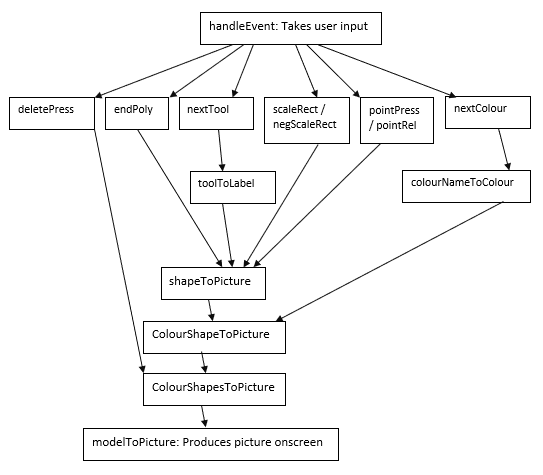
\includegraphics[width=0.85\textwidth]{program.png}\\
Function dependencies.
\end{center}
The top functions are from \verb|module Controller|, allowing user control of the model whilst the functions within  \verb|module View| produce an image from the model.

\subsection{Technical Decisions}
\textbf{Part 1} used case statements for all three functions as they were all injective with no need for guards.
 \textbf{Part 2} Whilst \verb|colourNameToColour| uses simple case matching, \verb|shapeToPicture| is more complicated, case matching on the tool it returns a CodeWorld \verb|Picture|. For both triangle and rectangle tools the \verb|solidPolygon| function was used to create the associated picture due to the specifications of the input not aligning well to a specific CodeWorld function. For the triangle the points used were the two given points and a third given by the function \verb|otherTriPoint| that calculated the other isosceles point. For rectangles the other two points are a translation of the first two points by a degree dictated by the scaling factor. Necessitated by the clip window and translations used, cap was guarded to determine if the cutoff was below the circle or not. If so it just returns a circle, otherwise the desired cap will be produced. \verb|colourShapeToPicture| used both prior part 2 functions and the CodeWorld  \verb|coloured| function to return a coloured picture. Finally it was necessary for  \verb|colourShapesToPicture| to recurse through the list of colourshapes as the list could be of any length.
 \textbf{Part 3} was a simple implementation. The main function \verb|handleEvent| cased on different inputs and would, instead of nesting cases, call appropriate helper function(s) which could case on the required part of the input to produce the desired output.  To reduce the risk of case non-exhaustion errors most helpers had a wildcard case.

 \subsection{Assumptions}%Describe assumptions you have made about how a user might use the program and how this has influenced your design decisions.
A specification gap for \verb|handleEvent| necessitated assuming that \verb|pointRel| should leave the scale factor of the rectangle tool unchanged upon the completion of a rectangle rather than re-initialise. This is hoped to reduce the amount a user has to change the scale factor to sequentially draw similar rectangles. For \verb|colourShapesToPicture| it was assumed that in case of an empty shapes list it should return a blank picture, and thus used the CodeWorld function \verb|blank|.

%~~~~~~~~~~~~~~~~~~~~~~~~~~~~~~~~~~~~~~~~~~~~~~~~~~~~~~~~~~~~~~~~~~~~~~~~~~~~~~~~~~~~~~~~~~~~~~~~~~~~

\section{Testing}%How did I test the program focus on methodology and testing groups
\paragraph{Part 1} 
 composed of three functions was tested using and passed the provided black-box test under \verb|cabal v2-test| indicating correctness. Further simple white-box tests were conducted within development calling functions with edge-case inputs in the terminal to ensure the case matching was error tolerant, eventually any such errors were deemed eliminated.
 
\paragraph{Parts 2 \& 3} 
were tested firstly by removing all compilation errors or warnings. As the Part 3 functions are designed to call the functions in both parts 1 and 2 it was decided it would be possible to test the functionality of parts 2 and 3 just through rigorous black-box testing of program GUI response. Each shape tool was tested in as many input configurations as possible including colour. Further all key inputs were tested to ensure they produced the desired response. The program passed both testing regimes. Finally, testing concluded with some white-box tests for edge case key inputs to check for crashes or specification violations. Firstly the delete command was tested on a blank canvas and did not have any unintended consequences. Next, various variations of capTool, the most complex tool, were tested in all four coordinate quadrants and various sizes. Key input responses were also tested when mid-drawing of a shape. Further, the functions in part 2 were subjected to a number of  supplementary Black-Box doctests all of which passed. Consequently as no errors could be found and everything held to specifications the program can be deemed correct.
%~~~~~~~~~~~~~~~~~~~~~~~~~~~~~~~~~~~~~~~~~~~~~~~~~~~~~~~~~~~~~~~~~~~~~~~~~~~~~~~~~~~~~~~~~~~~~~~~~~
\section{Reflection}
Due to the simple nature of and efficacy of the program the author does see any impetus to build the program differently. Further they did not run into any notable development issues or any strain on their technical skills. Due to its simplicity the code is easily interpreted and well documented.
%~~~~~~~~~~~~~~~~~~~~~~~~~~~~~~~~~~~~~~~~~~~~~~~~~~~~~~~~~~~~~~~~~~~~~ ~~~~~~~~~~~~~~~~~~~~~~~~~~~~~~~


%~~~~~~~~~~~~~~~~~~~~~~~~~~~~~~~~~~~~~~~~~~~~~~~~~~~~~~~~~~~~~~~~~~~~~~~~~~~~~~~~~~~~~~~~~~~~~~~~~~~~
\end{document}